% !TeX spellcheck = en_US
\addsection{Deckbuilding}{\skills/wisdom.png}

\begin{multicols*}{2}

\subsection*{\hypertarget{Playerdecks}{Player Decks}}
All players have a unique Deck which represents their Main Hero's Abilities and Equipment.
Decks may contain Statistic, Ability, Spell, Artifact and the Main Hero's Specialty Cards.

Each player's Deck starts with 9 cards, built during the game's setup.
This deck is called your \textbf{Deck of Might \& Magic}. From this point in this rule book this is \textbf{shorthanded} to \textbf{Your Deck}.
\subsection*{General Card Rules}
\begin{enumerate}
  \item Cards can be played \textbf{only on your Turn}, or in a \hyperlink{Combat}{Combat} involving your \textbf{Main Hero}.
  \item After a Card is used, discard it.
    Each player has their own separate Discard Pile for their own Deck.
  \item If Your Deck is empty when you need to draw a Card, \textbf{shuffle your Discard Pile} into a new Deck to draw from.
  \item Whenever a Hero gains a Card for any reason, put it \textbf{directly into your hand} unless otherwise stated.
  \item Whenever you are instructed to \textbf{Search} (X) the Ability, Artifact, or Spell Deck, you may either look at the top (X) Cards from the specified Deck, take one of them to your hand, and discard the others, \textbf{OR} instead of looking at the top (X) Cards, add the top Card from that Deck's Discard Pile to your hand.
  \item The Ability, Artifact, and Spell Decks each have their own Discard Piles, created during the setup, which help players identify these Decks.
    If a Deck ever runs out of Cards, reshuffle it and discard its top Card to form a new Discard Pile.
    Also, whenever one of these Discard Piles is empty, \textbf{refill it} with that deck's top Card.
  \item Cards in Your Deck have the following types of effects:
  \begin{itemize}
        \item \textbf{Instant} \includesvg[height=10px]{\svgs/instant.svg} Effects are resolved immediately and can be played out of turn during Combat.
        \item \textbf{Activation} \includesvg[height=10px]{\svgs/activation.svg} Effects must be played when Activating your own Unit in Combat.
        \item \textbf{Map} \includesvg[height=10px]{\svgs/map.svg} Effects cannot be used during Combat.
        \item \textbf{Ongoing} \includesvg[height=10px]{\svgs/ongoing.svg} Effects last until they are used up or until the player who played them starts their next Turn (whichever happens first).
        \item \textbf{Permanent} \includesvg[height=10px]{\svgs/permanent.svg} Cards stay in your play area until discarded or replaced.
          \textbf{Players may have only one permanent Card at a time}; playing another discards the first.
    \end{itemize}
\end{enumerate}

\vspace*{\fill}
\begin{center}
  \hspace{3em}
  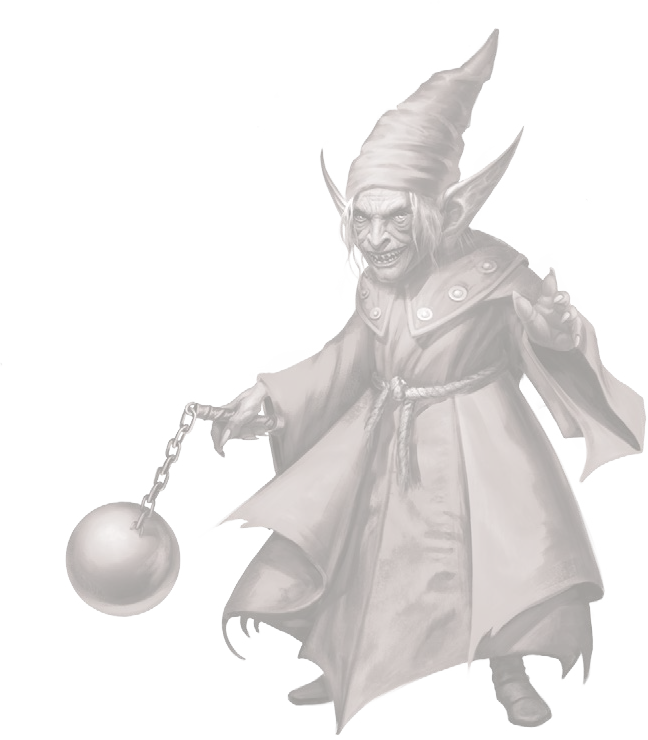
\includegraphics[width=0.8\linewidth]{\art/gremlin.png}
\end{center}

\clearpage

\subsection*{\hypertarget{Ability}{Ability and Statistic Cards}}

All Ability and Statistic cards have a Basic Effect and a stronger Expert \includesvg[height=10px]{\svgs/expert.svg} Effect, which is shown below the Basic Effect.
Whenever you play an Ability or Statistic card, you must choose which effect you are using.
The number of \includesvg[height=10px]{\svgs/expert.svg} Effects you can use each Round is limited by your Main Hero's \hyperlink{Level}{Level}.
Track the number of uses you have in any suitable manner, such as by moving Black Cubes on and off your Hero Card.\par
\bigskip

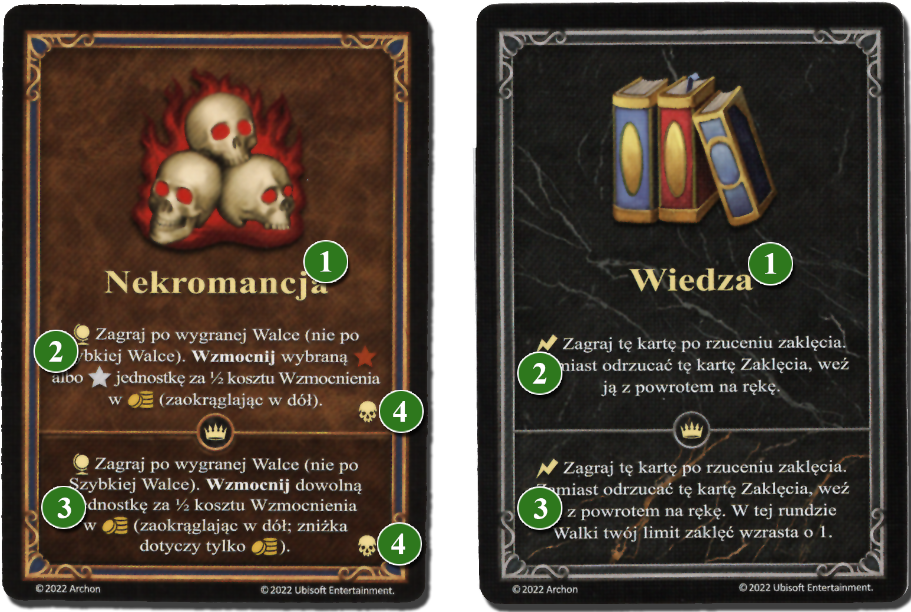
\includegraphics[width=\linewidth]{\cards/ability.png}

\note[big]{
  Certain cards are limited to the Necropolis Faction \includesvg[height=10px]{\svgs/necro-note.svg}.
  When a non-Necropolis player draws Necropolis Card from the Ability Deck, they may either discard it and draw a new Card as a replacement or gain it as normal.
  Non-Necropolis players \textbf{cannot use} Faction Specific Cards from their hand in any way besides for effects that discard them.
}

\subsection*{Artifact Cards}
Artifact Cards are divided into 3 Levels: Minor, Major, and Relic.
These Levels relate to the overall Power of the Card and may be referenced when resolving certain effects or during Scenario setup.
Otherwise, all Artifact Cards are normally shuffled together regardless of their Level.
Artifacts are gained through map exploration.\par
Artifacts can be \hyperlink{Trading}{traded} in Alliance and Cooperative Scenarios.\par
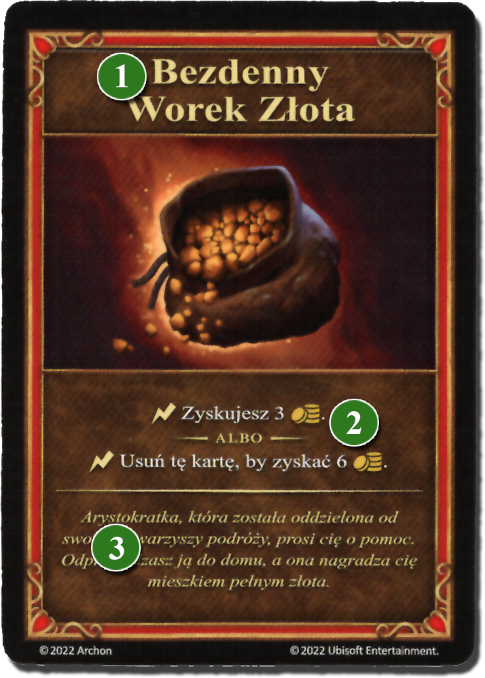
\includegraphics[width=\linewidth]{\cards/artifact.png}

\subsection*{\hypertarget{spells}{Spell Cards}}


Spell Cards have three possible primary effects.
Using the topmost, basic version of the Spell has no additional costs.
To access the other effects, you may \textbf{Empower} a Spell by paying the indicated cost (3) to get a more powerful outcome (4).
You may pay this cost by playing other cards for their Empower \includesvg[height=10px]{\svgs/empower.svg} effect before casting the Spell.
All Spell Cards also have an alternative bottom (5) \includesvg[height=10px]{\svgs/empower.svg} effect.\par

\filbreak
\begin{center}
  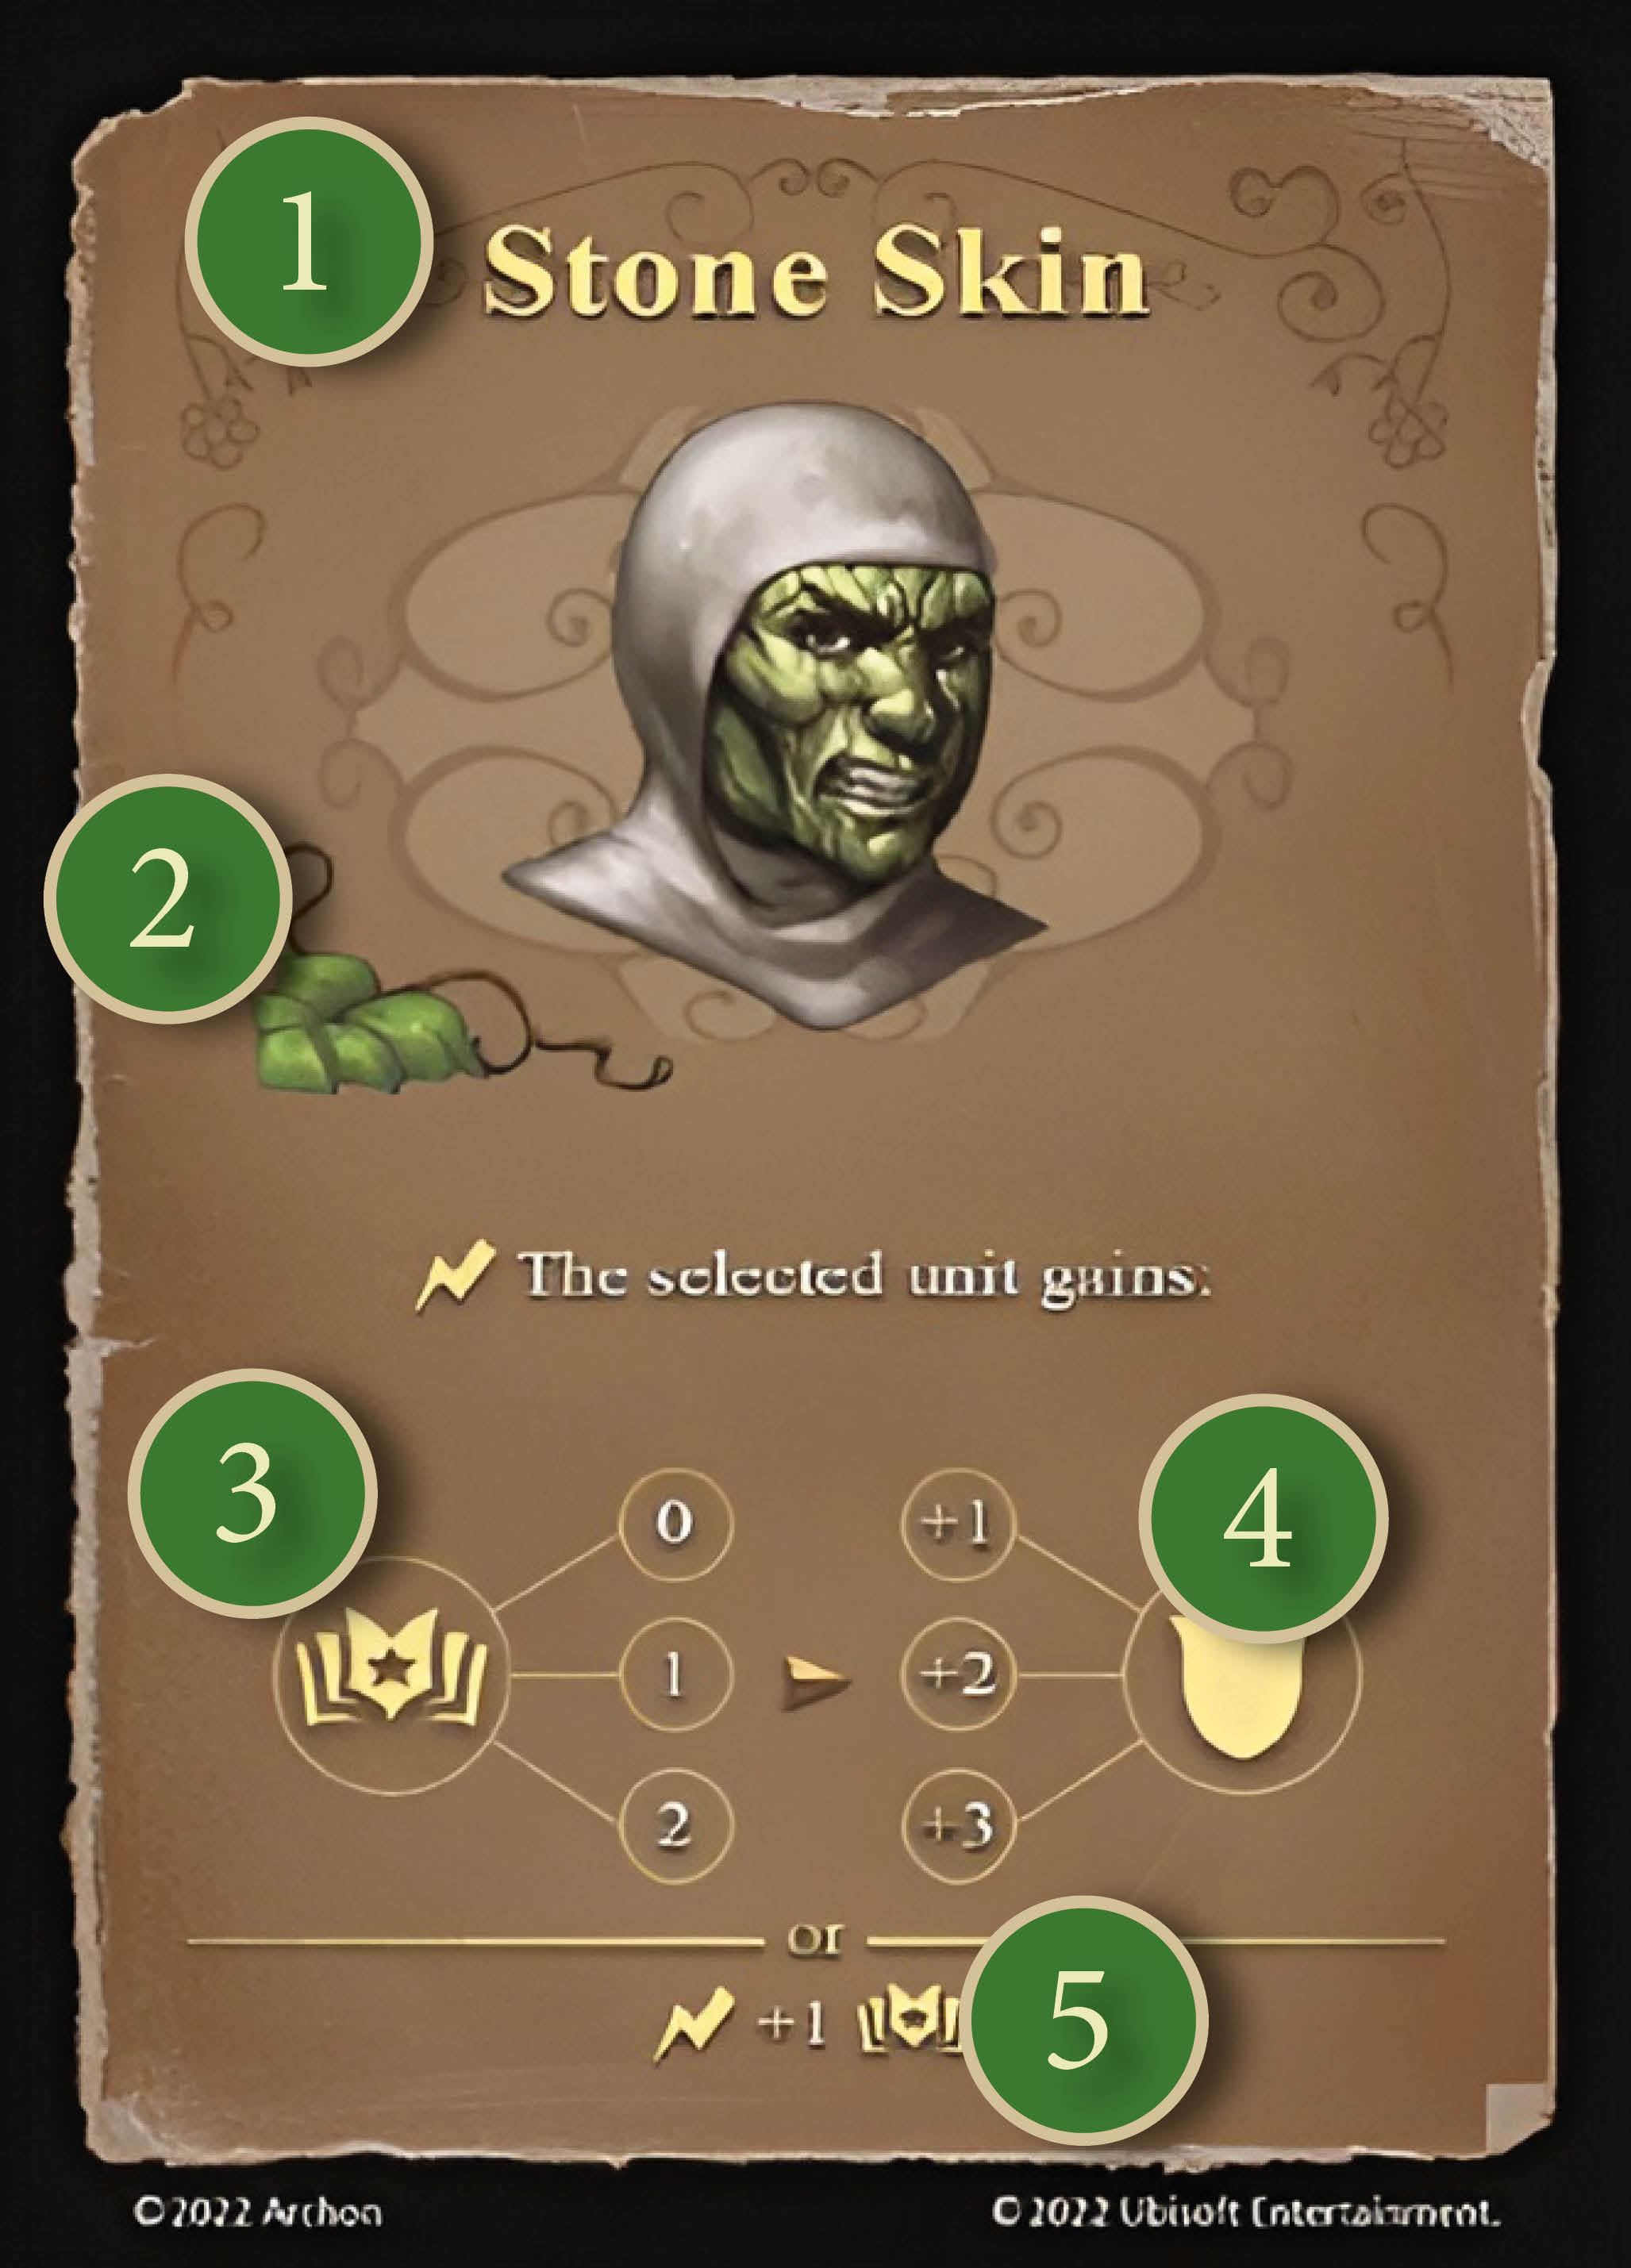
\includegraphics[width=0.6\linewidth]{\cards/spell_example.jpg}\\
  \medskip
  \footnotesize{\textbf{\textit{\textcolor{darkcandyapplered}{Spell Card}}}}
  \scriptsize
  \begin{multicols}{2}
    \begin{itemize}[itemsep=5pt]
      \item[\textbf{1.}] \textbf{Spell Name}
      \item[\textbf{2.}] \textbf{School of Magic}
      \item[\textbf{3.}] \textbf{Cost to Empower}
      \item[\textbf{4.}] \textbf{Spell Effect}
      \item[\textbf{5.}] \textbf{Alternative Effect}
      \item[]
    \end{itemize}
  \end{multicols}
\end{center}

\note{During Combat, \textbf{only one Spell Card} may be played by each player \textbf{per Combat Round}.}\par
Spells can be gained by Building the Mage Guild.
When you do, \textbf{Search} (2) the Spell Deck, \textbf{twice}.
If you start a Scenario with the Mage Guild, perform the searching in Turn order and shuffle the Cards you gained into your Deck at the end of the setup.\par
More Spells can be bought by flipping your Spell Book Token and paying the indicated cost on the Mage Guild to \textbf{Search} (2) the Spell Deck.
This cannot be done during the \textbf{same Round} as when the Guild is constructed.\par
Spells can be \hyperlink{Trading}{traded} in Alliance and Cooperative Scenarios.

\subsection*{\hypertarget{Specialty}{Hero Specialty Cards}}

Hero Specialty Cards are gained from \hyperlink{Level}{Level ups}.
Each Main Hero has an unique set of them.
While many Specialty Cards have effects which resemble Spell Cards, Specialty Cards are their \textbf{own unique category of card}, which are not affected by effects that do not specify them.

\begin{center}
  \shadowimage[width=0.6\linewidth]{\cards/specialty.jpg}\\
  \medskip
  \scriptsize\textit{A Level 4 Specialty Card, belonging to Catherine the Knight.}
\end{center}

\subsection*{Example}

\textit{Deemer the Warlock has built a Mage Guild during the previous Game Round, enabling him to now use his Spell Book Token to purchase additional Spells.
He spends the token and pays the cost indicated on his Town Board, allowing him to \textbf{Search (2)} the Spell Deck.}\par
\textit{He now has the choice of either gaining the top Card of the Spell Card Discard Pile, or drawing the top two Cards of the Spell Deck and gaining one of them.
He is not interested in gaining the Spell Curse, which is on top of the Discard Pile, and instead decides to draw two Cards – a Magic Arrow and a Fireball.
He decides to keep the Fireball, placing it into his hand and discarding the Magic Arrow into the Spell Discard Pile.}

\end{multicols*}
